\section{Meta-learning mesh-free PDE operators}
We consider time-dependent PDEs
\begin{align}
\frac{\partial}{\partial t}u(\bm{x}, t) + \mathcal{N}\left[ u(\bm{x}, t)\right] &= 0 &\bm{x} \in \Omega, t \in [0, T], \label{eq:metapde-time-strongform} \\
G(u)(\bm{x}, t) &= 0 & \bm{x} \in \partial\Omega, t \in [0, T], \label{eq:metapde-time-bc} \\
u(\bm{x}, 0) &= \bar{u}_0(\bm{x}) &\bm{x} \in \Omega, t=0, \label{eq:metapde-time-ic} 
\end{align}
as well as time-independent PDEs which only have spatial dependence:
\begin{align}
\mathcal{N}\left[ u(\bm{x})\right] &= 0 & \bm{x} \in \Omega, \label{eq:metapde-space-strongform} \\
G(u)(\bm{x}) &= 0 & \bm{x} \in \partial\Omega. \label{eq:metapde-space-bc}
\end{align}
The problem is defined on the spatial domain $\Omega \subset \mathbb{R}^{d}$ with boundary $\partial \Omega$. For time-dependent PDEs the time horizon is $[0, T]$. 
%The unknown function in the PDE $u(\bm{x}, t)$ is a function of the spatial coordinate $\bm{x}$ and time coordinate $t$. 
%$\partial / \partial t u(\bm{x}, t) $ is the partial derivative of the unknown function $u$ with respect to the time. 
%$\mathcal{N}\left[ u(\bm{x}, t)\right]: (\Omega \to \mathbb{R}^{d_u}) \to (\Omega \to \mathbb{R}^{d_\mathcal{F}})$ is an operator that involves $u$ and the partial derivatives of $u$ with respect to its spatial coordinates $\bm{x}$.
In both cases $\mathcal{N}$ is an operator that involves $u$ and the partial derivatives of $u$ with respect to its spatial coordinates $\bm{x}$.

%Figure \ref{fig:metapde-poisson} shows as an example the Poisson problem on a disc. For this simple problem we have $\mathcal{F}(u) = \nabla^2 u - f$, for a spatially varying source term $f$, and $\mathcal{G}(u) = u$, i.e. enforcing $u=0$ on the boundary. 
%\begin{figure}[t]
%  \centering
%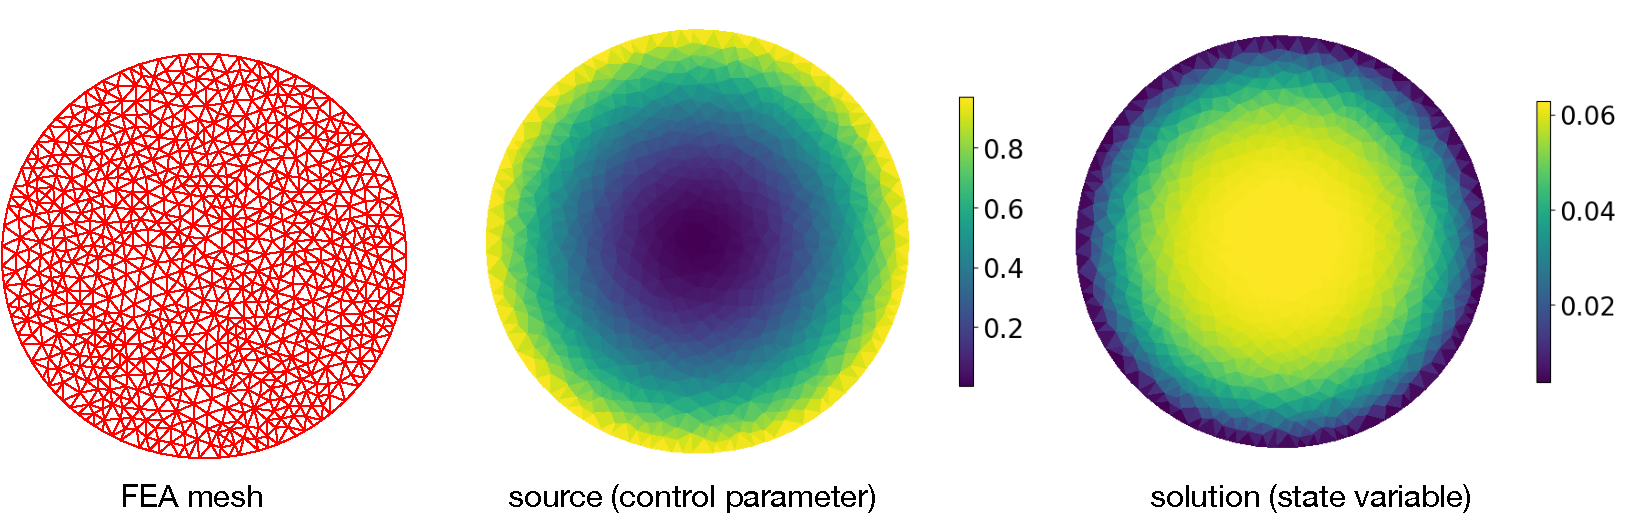
\includegraphics[width=0.8\linewidth]{figures/poisson_equation.pdf}
%\caption{Poisson equation on a disc.
%Figure: \citet{xue2020amortized}.}%
%\label{fig:metapde-poisson}%
%\end{figure} \\
\subsection{Physics-Informed Neural Networks (PINN)}
The goal of a PINN is to represent the solution ansatz $u(\bm{x},t)$ with a neural network $f_\theta(\bm{x},t)$. 
Doing so requires learning $\theta$ such that $f_\theta$ approximates the solution to the PDE over the problem domain.
Learning these parameters is an optimization problem, which requires defining a loss function whose minimum is the solution of the PDE.
%In the original proposal, PINNs can not only incorporate the standard "supervised" data loss, but also a physics-informed loss. 
%The standard supervised loss requires knowing the ground truth solution evaluated at sample points. 
%This "supervised" data loss is useful when experimental data is available. 
%The physics-informed loss consists of the residual of the differential equation. 
%Therefore, one way to incorporate the is to minimize the residual when using $f_\theta$ as the ansatz to the PDE solution $u$. 
We choose a `physics-informed loss' which consists of the residual of the differential equation over the problem domain and boundary. For time-independent PDEs, this loss function is
\begin{align}\label{eq:pinn_loss_function}
  \mathcal{J}(u) &= \int_{\Omega} \left|\left| \mathcal{N}(u)(\bm{x})\right|\right|^2_2 \, dx + \int_{\partial\Omega} \left|\left| \mathcal{G}(u)(\bm{x})\right|\right| _2^2 \, dx.
\end{align}
For time-dependent PDEs, this loss function is: 
\begin{align}\label{eq:pinn_loss_function}
  \mathcal{J}(u) = & \int_{\Omega} \left|\left| \frac{\partial}{\partial t}u(\bm{x}, t) + \mathcal{N}(u)(\bm{x}, t)\right|\right|^2_2 \, dx + \\
  & \int_{\partial\Omega} \left|\left| \mathcal{G}(u)(\bm{x}, t)\right|\right| _2^2 \, dx + \int_{\Omega} \left|\left| u(\bm{x}, 0) - \bar{u}_0(\bm{x}) \right|\right| _2^2 \, dx .
\end{align}
During training, we randomly sample collocation points from the PDE domain $\Omega$ and boundary $\partial \Omega$ and use these points $\mathcal{C} \in \Omega$ and $\partial \mathcal{C} \in \partial \Omega$ to approximate the differential equation residual. For time-independent PDEs, the training loss is
\begin{align}\label{eq:pinn_training_loss}
    \mathcal{L}_{\text{PINN}}(f_\theta) = \frac{1}{|\mathcal{C}|} \sum_{\bm{x} \in \mathcal{C}} \left|\left| \mathcal{N} (f_{\theta})(\bm{x}) \right|\right|_2^2  + \frac{1}{|\partial \mathcal{C}|}  \sum_{{\bm{x} \in \mathcal{\partial \mathcal{C}}} } \left|\left|\mathcal{G}(f_{\theta})(\bm{x})\right|\right|_2^2.
\end{align}
For time-dependent PDEs, the training loss is
\begin{align}\label{eq:pinn_training_loss}
    \mathcal{L}_{\text{PINN}}(f_\theta) = & \frac{1}{|\mathcal{C}|} \sum_{\bm{x} \in \mathcal{C}}\left|\left| \frac{\partial}{\partial t}(f_\theta)(\bm{x}, t) + \mathcal{N} (f_{\theta})(\bm{x}, t) \right|\right|_2^2  +\\ 
     & \frac{1}{|\partial \mathcal{C}|}  \sum_{{\bm{x} \in \mathcal{\partial \mathcal{C}}} } \left|\left|\mathcal{G}(f_{\theta})(\bm{x}, t)\right|\right|_2^2 + \frac{1}{|\mathcal{C}|} \sum_{\bm{x} \in \mathcal{C}} \left|\left| f_{\theta}(\bm{x}, 0) - \bar{u}_0(\bm{x}) \right|\right| _2^2.
\end{align}

When the training converges, we expect $f_{\theta}$ to approximately satisfy the above equations, meaning that $\mathcal{L}_{\text{PINN}}(f_\theta)$ should be nearly zero.
%As with \citet{xue2020amortized}, we use this optimization perspective to derive an efficient training method for our surrogate models.

\subsection{Meta-PDE Method}

This lets us develop a new, ``functional'' API for surrogate modeling.
%, which can handle arbitrary geometries and removes the need to fix a mesh or to fix vector bases for the PDE parameters or solution.
For a given PDE, our surrogate model takes as input: 
\begin{itemize}
    \item[(i)] Samplers which can sample points uniformly on each region of the domain.
    \item[(ii)] A loss function encoding the PDE constraint or boundary condition for each such region.
\end{itemize}
Combining these allows estimation of the residual which measures deviation of a given solution field from the governing equations. We use a neural network to model the solution field, and train a neural network initialization to converge quickly across a distribution of tasks; in our case each task in the distribution is minimizing the residual for a PDE or minimizing the variational energy for the PDE with given domain, boundary conditions and governing equations. 

In this work, we use gradient-based meta-learning to amortize the training time needed to fit each parametrization of the PDE. The LEAP-based Meta-PDE method learns the model initialization $\theta^0$ for a neural network $f_\theta$. $f_\theta$ can be trained to approximate the solution $u: \mathbb{R}^{d_\Omega} \to \mathbb{R}^{d_u}$ of an individual parametrization of the PDE. To learn $\theta^0$, we start with a distribution of tasks, with each task specified by samplers and constraint operators for the boundary and loss. Each task in this distribution represents a different parametrization of the PDE. Then we draw a batch of $n$ tasks with individual loss functions $\hat{\mathcal{L}}_i$, $i \in [n]$. The initialization for each inner task is $\theta^0$, and is updated by the inner gradient update rule. During each inner gradient update, we update the meta-gradient per LEAP algorithm. We unroll the inner learning loop $K$ steps to find $f_{\theta_i^K}$: the solution ansatz for each task $i$ in the batch. After unrolling $K$ update steps for $n$ tasks, we update the learned model initialization $\theta^0$ with the meta-gradient:
\begin{align}
    \theta^0 \leftarrow \theta^0 - \beta \nabla_{\theta^0}\sum_{i=1}^n \frac{1}{n} d(\theta^0; M_i),
\end{align}
where $d(\theta^0; M_i)$ is the distance of the gradient path for task $i$ on its manifold $M_i$, as specified in \citep{flennerhag2018transferring}.

The MAML-based Meta-PDE method learns the model initialization $\theta^0$ for a neural network $f_\theta$ and also learns the inner gradient update rule. We use SGD as the inner gradient update rule and MAML learns the optimal step size for each parameter in $\theta$ for each inner each step. For each task the loss is $\hat{\mathcal{L}}_i(f_{\theta_K, i})$. We perform backpropagation through the inner loop to find the gradients w.r.t meta-initialization $\theta_0$ and use the gradients to update $\theta_0$ in the outer loop training:
\begin{align}
    \theta^0 \leftarrow \theta^0 - \beta \nabla_{\theta^0} \sum_{i=1}^n  \frac{1}{n} \hat{\mathcal{L}}_i(f_{\theta^K _i})
\end{align}
We also perform backpropagation through the inner loop to find the gradients w.r.t. the per-step, per-parameter step size $\alpha$ and use the gradients to update the $\alpha$ in the outer loop training:
\begin{align}
    {\alpha}  \leftarrow {\alpha} - \beta  \nabla_{\alpha} \sum_{i=1}^n  \frac{1}{n} \hat{\mathcal{L}}_i(f_{\theta^K_i})
\end{align}

The Meta-PDE surrogate model is designed to have an input schema as close to this general specification as possible. Most PDEs can be fully defined by specification of:
\begin{itemize}
  \item a domain $\Omega$ with boundary $\partial \Omega$,
  \item an operator $\mathcal{F}$ representing governing equations,
  \item and an operator $\mathcal{G}$ representing boundary conditions.
\end{itemize}
When using Meta-PDE as a surrogate to compute an approximate solution to a given paramterization of the PDE (one task), the inputs to the Meta-PDE model immitate the general. specification above:
\begin{itemize}
  \item a sampler $s(\Omega)$ which returns points in the domain $\Omega$,
  \item a sampler $s(\partial\Omega)$ which returns points on the boundary $\partial\Omega$,
  \item an operator $\mathcal{F}$ representing governing equations,
  \item and an operator $\mathcal{G}$ representing boundary conditions.
\end{itemize}
The operators $\mathcal{F}$ and $\mathcal{G}$ may be supplied directly and do not require a particular parametric form. The geometric dimension $\mathbb{R}^{d_\Omega}$ and solution dimension $\mathbb{R}^{d_u}$ must remain fixed across PDEs in the distribution, even though $\Omega$ is allowed to vary. The samplers and operators are sufficient to construct an estimator $\hat{\mathcal{L}}$ for the task loss $\mathcal{L}$:
\begin{align}
  \mathcal{L}(u) &= \int_{\Omega} \big|\big|\mathcal{F}(u)(\bm{x})\big|\big|^2_2 d\bm{x} +
  \int_{\partial\Omega} \big|\big|\mathcal{G}(u)(x)\big|\big|_2^2 d\bm{x} \\
  \hat{\mathcal{L}}(u) &= \mathbb{E}_{x \sim s(\Omega)} \big|\big|\mathcal{F}(u)(\bm{x})\big|\big|^2_2 +
  \mathbb{E}_{\bm{x} \sim s(\partial \Omega)} \big|\big|\mathcal{G}(u)(\bm{x})\big|\big|_2^2
\end{align}
$\hat{\mathcal{L}}(f)$ is unbiased as long as $s(\cdot)$ return points with uniform probability over their supports, or return batches of points which have uniform probability for any given $x$ aggregated over the batch. Unbiased estimation is not necessarily essential. Note $\hat{\mathcal{L}}(f) > 0$ and $\mathcal{L}(f) > 0$ $\forall f$, and the true solution $u$ of the PDE achieves $\mathcal{L}(u) = \hat{\mathcal{L}}(u) = 0$. These properties hold if we multiply the integrand in $\mathcal{L}(f)$ by an arbitrary density $\mu > 0$ or if we choose samplers $s$ which have full support but nonuniform probability on $\Omega$ or $\partial \Omega$. Therefore, biased sampling will not change the minimizer of the energy estimator if we have a sufficiently expressive hypothesis class for $f$.

%The user must supply a sampler for the domain and for the boundary of each PDE within the training distribution and for each PDE seen during deployment. A sampler can easily be constructed for any domain for which we have a mesh, but it is also often easier to construct a sampler than to construct an accurate mesh.
During deployment time, a "forward pass" computes an approximate solution for a given PDE parametrization with $K$ steps of stochastic optimization steps. The $K$ gradient steps minimize the residual for the task $\mathcal{L}(f)$. If the model has been trained with LEAP-based Meta-PDE method, it will start from the meta-learned model initialization $\theta_0$. If the model has been trained with MAML-based Meta-PDE method, it will start from the meta-learned model initialization $\theta_0$ and the step size $\alpha$ will be also be specified for each parameter and each step: 
\begin{align}
  \theta^k = \theta^{k-1} - \alpha \nabla_{\theta^{k-1}} \hat{\mathcal{L}}(f_{\theta^{k-1}}) \quad k = 1 .. K
\end{align}
In both cases, the Meta-PDE method returns the approximate solution $f_{\theta^K}$, the neural network with the final set of parameters. One could further fine tune the model beyond $K$ gradient steps to achieve higher solution accuracy at the cost of longer solving time. 

Finite element analysis methods usually use piecewise linear meshes, which can take many elements to accurately represent curved shapes: even when using piecewise polynomially-shaped meshes, the slow rate of convergence of using these meshes to approximate non-polynomial geometry can be a major source of error and/or computational expense for FEA. In the next section, we will further explore the accuracy/time trade-off for Meta-PDE during deployment, and compare it with the accuracy/time trade-off for FEA methods. 

%Given an inside-outside oracle for the domain, it is easy to use rejection sampling to sample from it exactly. Most parametric geometry representations such as those used in computer-aided design also allow exact sampling of the boundary, and even minimal representations such as signed distance functions allow approximate sampling \citep{brubaker2012family}.
